\section{概览}
本文的背景技术分析部分介绍了当前的动态分析相关技术和实现工具以及Android系统的部分运行原理\juhao 结合前面的分析和系统实现的可行性, 本系统整体实现方案如下:

采用\ref{artInstr}节提到的ART Instrumentation的技术, 修改Android8.1系统源代码中ART虚拟机部分来实现Java层次的方法调用监控和简单的脱壳功能\juhao 通过Frida工具来实现对本地函数调用以及Java层特定方法的监控, 同时增加监控系统的灵活性和可扩展性\juhao 修改Android源代码中与应用启动相关的部分实现监控应用的启动情况, 在目标应用启动时开启其他监控功能\juhao 通过简化日志内容和使用内存缓存日志的方式实现更为高效的日志系统用于保存监控系统记录的数据\juhao 通过系统属性来实现目标应用和其他配置选项的设置\juhao 

图\ref{emOverview}描述了系统的总体设计, 加粗的矩形部分为本系统的模块\juhao 其中EvMonitor-core模块运行在ART内部, 负责监控Java方法调用, dex文件解析, 并且实现了日志系统\juhao 该部分还通过JNI给运行在应用层的EvMonitor-startLogger模块提供了接口, 可以启动和关闭监控功能, 调用日志系统等, 这些接口也通过导出函数的方式提供给EvMonitor-Frida调用\juhao EvMonitor-Frida是一个本地动态链接库, 用于实现对本地层函数调用以及某些特别感兴趣的Java层方法的监控, 在目标应用进程加载应用文件之前被加载到目标进程中, 开启对目标应用的监控\juhao 
\begin{figure}[ht]
	\centering
	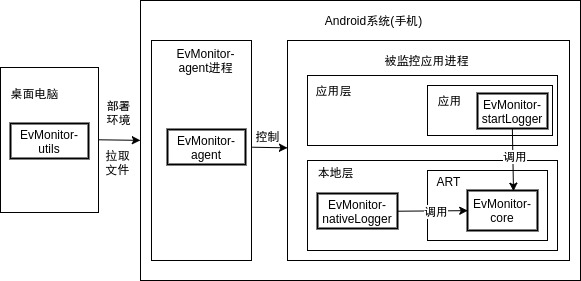
\includegraphics[width=\textwidth]{em_overview.jpg}
	\caption{EvMonitor概览}
	\label{emOverview}
\end{figure}

\section{监控应用启动}
本功能由EvMonitor-startLogger实现\juhao 
\ref{appStartA}节详细介绍了Android系统应用的启动过程\juhao 由于Android应用进程不是通过直接使用应用APK文件启动, 而是通过Zygote进程fork产生, 因此无法按照传统PC上启动子进程, 然后加载监控模块开启监控, 最后再加载目标应用开始执行的方式来实现在应用加载前启动对应用的监控\juhao 只有通过监控应用的启动, 在能够获取到应用的名称并且应用自身代码还未执行时开启完成监控应用的初始化操作\juhao ActivityThread类的handleBindApplication方法开始的位置符合上述条件, 因此本系统选择在handleBindApplication方法的适当位置添加监控代码\juhao 

监控代码的实现逻辑如下:
首先读取当前进程名和应用名(有些应用会启动多个进程), 使用日志系统记录当前启动的应用名和进程名\juhao 接着读取系统属性em.target\_type, 确定是只监控某个进程还是监控该应用的全部进程\juhao 接着根据上述结果读取系统属性获取要监控的进程名或者应用名并同本进程或者应用名比较, 如果不同则退出监控代码, 不启动监控系统; 如果相同则调用Evmonitor-core提供的初始化监控的接口来启动对该应用的监控\juhao 之后再根据当前运行环境是32位还是64位加载对应的EvMonitor-Frida动态链接库, 完成监控系统的初始化\juhao 

为了便于调用JNI和被调用, 我将上述监控代码作为一个新的静态方法logAppStartAndSetTarget\_em加入了com.android.internal.os.Zygote类中, 并通过在Zygote类中增加本地方法nativeEnableMonitor的方式调用了EvMonitor-core提供的本地层接口\juhao 

\section{监控Java方法调用}
本功能由EvMonitor-core实现\juhao 
为了能够获取到应用所有Java方法调用行为, 本系统选择在ART内执行方法的函数中加入监控代码\juhao  \ref{methodExecA}节详细介绍了ART虚拟机执行方法的过程\juhao 根据分析, 在ArtMethod::Invoke和Execute函数中插入监控代码就能够记录所有的Java方法调用情况\juhao  

ART虚拟机中的每个Java方法都使用一个ArtMethod类型的对象来表示, 而在ArtMethod::Invoke和Execute执行方法时都能够获取到代表正在执行的方法的ArtMethod对象, 因此本系统在ArtMethod类(/art/runtime/artmethod.cc)中加入一个方法log\_em用于记录当前方法并写入日志中\juhao log\_em方法会调用当前ArtMethod对象的PrettyMethod方法获取方法信息然后调用EvMonitor-core中的日志系统将其写入日志\juhao 

本系统在ArtMethod::Invoke和Execute函数的入口和所有出口位置调用了上述log\_em函数记录方法执行的开始和结束\juhao 

\section{监控本地函数调用}
本功能由EvMonitor-Frida实现\juhao 本系统使用Frida工具的动态链接库形式(frida-gadget), 通过在应用加载自身代码之前加载frida-gadget并执行监控代码来实现对本地层函数调用的监控\juhao 目前的监控较为简单, 主要是利用了Frida工具提供的Interceptor来hook了open\dunhao execve\dunhao socket\dunhao dlopen\dunhao dlsym函数来监控它们的调用情况\juhao 由于Frida工具实现了Javascript的API, 因此可以灵活的添加监控函数和其他监控逻辑, 增强本系统\juhao 


\section{脱壳功能}
本功能由EvMonitor-core实现\juhao 
目前Android平台应用加固工具的加壳机制十分复杂, 本系统根据\ref{classLoadA}节介绍的类加载过程, 通过在用于dex文件加载的关键函数, 即位于安卓源代码中/art/runtime/DexFile.cc中DexFile类的构造函数DexFile()中加入代码来实现简单脱壳获取dex文件的功能\juhao 
DexFile类的构造函数原型图\ref{dexFileCode}所示\juhao 
\begin{figure}[ht]
	\centering
	\fbox{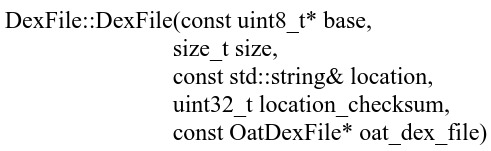
\includegraphics[width=8cm]{dex_file_code.jpg}}
	\caption{DexFile()原型}
	\label{dexFileCode}
\end{figure}
其中第一个参数是dex文件被加载到内存的起始地址, 第二个dex文件的大小\juhao 本系统插入该函数的监控代码会先检查是否开启对当前进程的监控, 如果监控功能没有开启则不在执行后续操作\juhao 如果监控功能开启会先调用日志系统记录当前加载的dex文件起始地址和大小, 然后再检查是否启动脱壳功能\juhao 如果脱壳功能启动则读取这两个参数后会调用EvMonitor-core中用于保存dex文件的dumpDex函数, 将加载的dex文件写入初始化时设定的位置\juhao 


\section{日志系统}
本功能由EvMonitor-core实现\juhao 各种动态分析系统中, 输入监控记录都是一个十分重要的功能, 但由于IO的速度很慢, 在频繁的调用中记录日志信息对应用本身的执行速度影响很大\juhao 在最初的测试中本系统使用Android系统本身的日志系统接口来记录监控信息, 但在测试中发现Java层方法的调用很多, 通过Android系统本身的日志系统输出会导致应用运行变得非常慢, 所以开发了本系统的日志部分\juhao 

表\ref{logValue}描述了日志系统用到的一些变量和提供的接口函数\juhao 
% Please add the following required packages to your document preamble:
% \usepackage{multirow}
\begin{table}[ht]
	\centering
	\caption{日志系统变量和函数}
	\begin{tabular}{cll}
		\hline
		\multicolumn{1}{l}{}                             & \textbf{名称}       & \textbf{作用}     \\ \hline
		\multirow{4}{*}{\textbf{变量}}                     & log\_base         & 记录日志缓冲区起始地址     \\
		& log\_data         & 记录日志缓冲区空闲区起始地址  \\
		& log\_spare\_space & 记录日志缓冲区空闲空间     \\
		& log\_file\_amount & 记录已经写入磁盘的日志文件数量 \\ \hline
		\multicolumn{1}{l}{\multirow{2}{*}{\textbf{函数}}} & log()             & 写入日志            \\
		\multicolumn{1}{l}{}                             & writeLog()        & 把缓冲区日志写入文件      \\ \hline
	\end{tabular}
\label{logValue}
\end{table}
日志系统会在初始化时使用mmap创建一个4M的内存缓冲区, 并在被监控应用的目录下以当前时间和进程号创建一个文件夹用来保存此次执行时的日志数据\juhao 缓冲区的起始地址会使用log\_base来记录, 并且log\_data会被初始化为同log\_base一致\juhao 
当log函数被调用来记录日志时, 其会先检查log\_spare\_space, 如果空间足够就会把接收到的日志信息加上当前线程号写入log\_data位置处的内存缓冲区中并更新log\_spare\_space\dunhao log\_data的值 \juhao 如果空间不足就会调用writeLog函数试图把缓冲区的日志写入文件\juhao writeLog函数会检查log\_file\_amount的值确定日志文件数量是否达到最大, 如果是, 则通过Android系统的log系统记录一个日志文件以达到数量上限的错误, 并不在执行后续操作, 如果不是则将缓冲区的数据写入文件, 并将log\_base的值赋给log\_data, 设置log\_spare\_space的值为缓冲区最大容量, 同时把log\_file\_amount加1\juhao 

